\chapter{Progettazione concettuale}

\begin{figure}[hbt]
\section{Class Diagram}
\centering
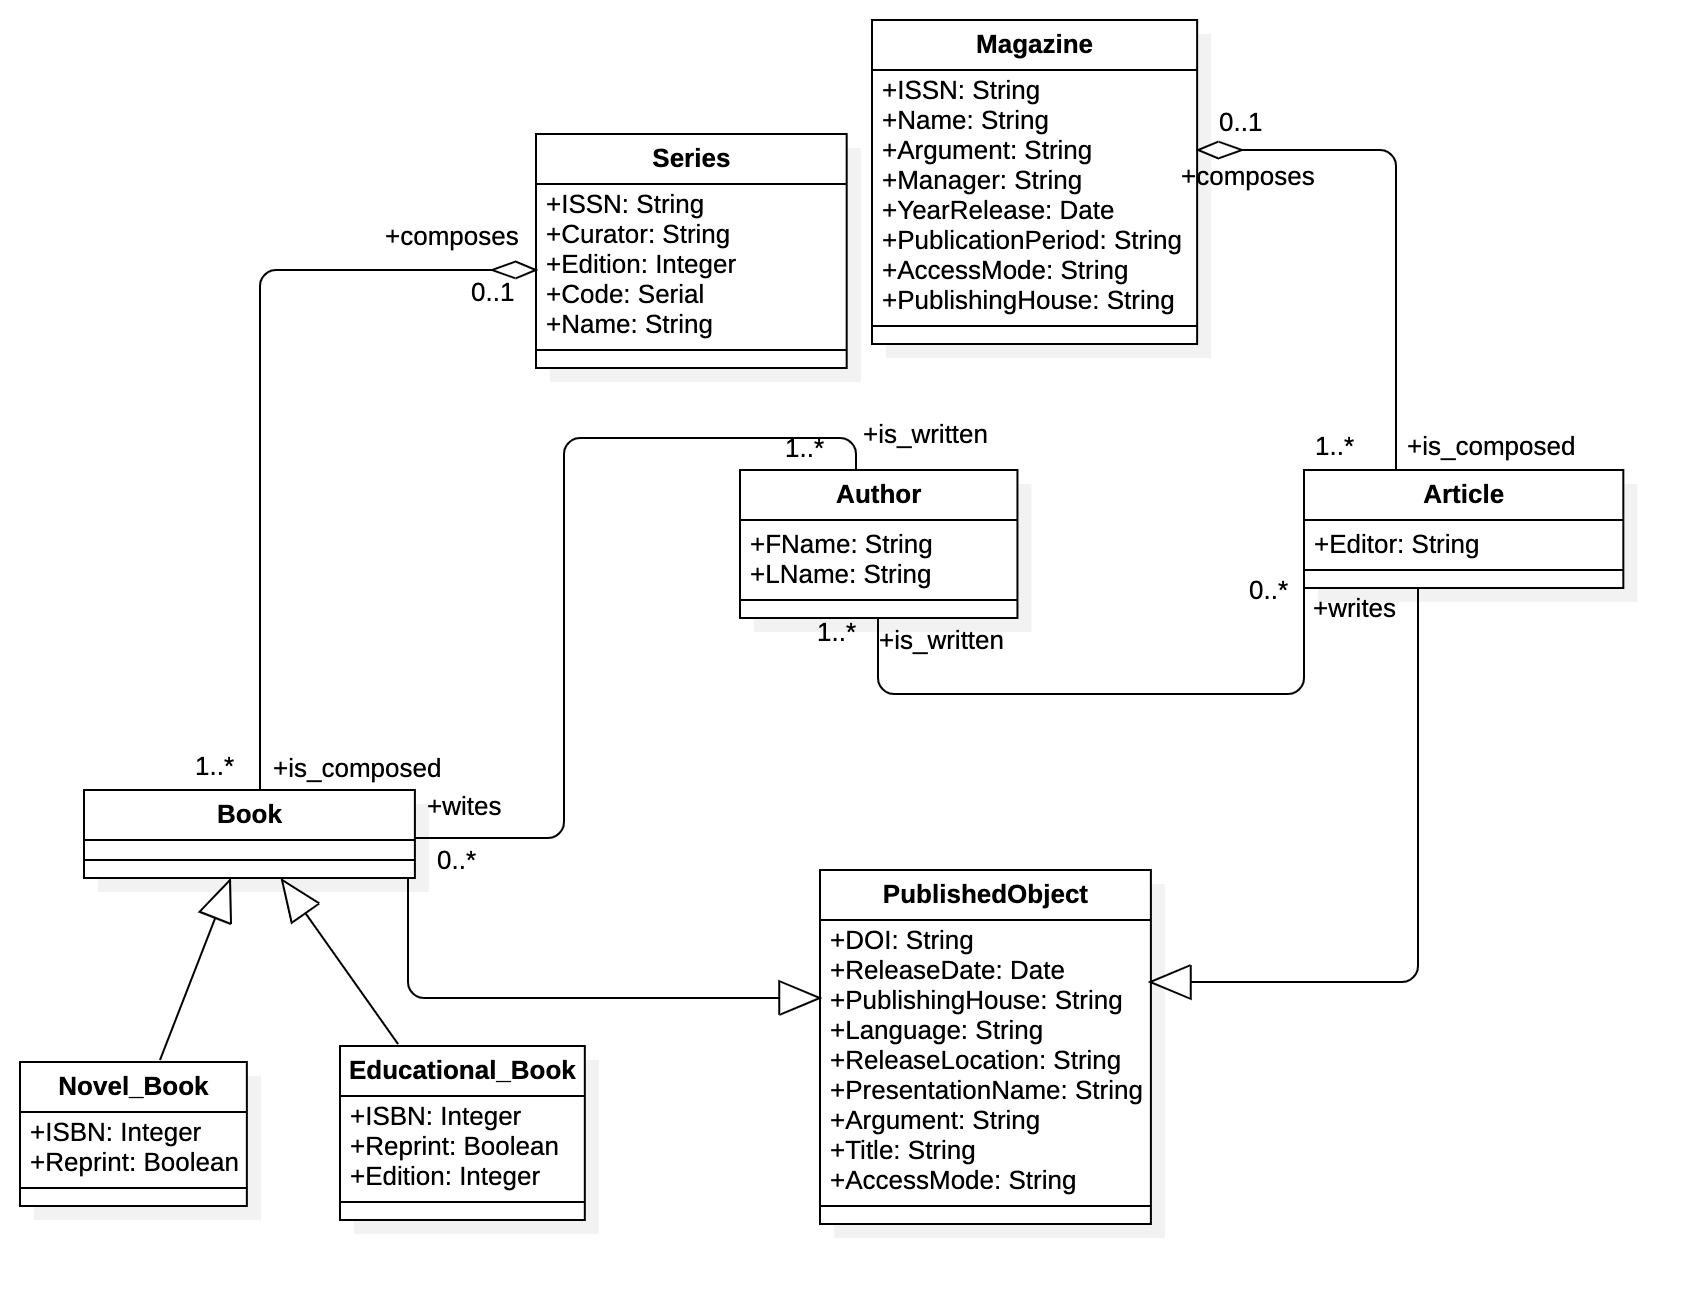
\includegraphics[width=1.1\textwidth]{Immagini/ClassDiagram.png}
\caption{Class Diagram}
\label{fig:ClassDiagram}
\end{figure}

\section{Analisi della ristrutturazione del Class Diagram}

\subsection{Analisi delle ridondanze}

Le ridondanze individuate nell class diagram sono presenti nella specializzazione della classe \texttt{Book} in: \texttt{Novel\_Book} e \texttt{Educational\_Book}. \\ 
Gli attributi: \texttt{ISBN} e \texttt{Reprint} di entrambe le specializzazioni vengono inserite all'interno della classe \texttt{Book}.

\subsection{Analisi degli identificativi}
Identificativo primario per la classe \texttt{Book} è l'attributo \texttt{DOI}, viene attribuito all'attributo \texttt{ISBN} il vincolo di chiave candidata. 
Per la classe \texttt{Author} viene implementato un attributo aggiuntivo: \texttt{ID\_Author} che sarà chiave primaria.
Per la classe \texttt{Article} viene usato l'attributo \texttt{DOI} come chiave primaria.
Per le classi \texttt{Series} e \texttt{Magazine} viene usato come chiave primaria l'attributo \texttt{ISSN}.

\subsection{Rimozione degli attributi multipli}
Non sono presenti attributi multipli all'interno del Class Diagram.
\subsection{Rimozione degli attributi composti}
Non sono presenti attributi composti all'interno del Class Diagram.

\subsection{Partizione/Accorpamento delle associazioni}
In questo Class Diagram non sono presenti associazioni 1..1 da eliminare.
\subsection{Rimozione delle gerarchie, delle composizioni}
Nel Class Diagram vengono incorporati nella classe \texttt{Book} le specializzazioni \texttt{Novel\_Book} e \texttt{Educational\_Book} assieme ai rispettivi attributi. All'attributo \texttt{Argument} nel Class Diagram ristrutturato, viene specificato l'argomento educativo (Filosofia, Economia ecc.) oppure all'attributo viene assegnato il valore: Romanzo.\\
Dato l'interesse di tracciamento delle classi \texttt{Book} e \texttt{Article} in modo separato, viene eliminata la classe \texttt{PublishedObject} e i suoi attributi vengono inseriti all'interno delle classi menzionate precedentemente.
Le composizioni che riguardano le classi \texttt{Series} e \texttt{Magazine}, vengono eliminate e sostituite da una semplice associazione.
\newpage
\section{Class Diagram ristrutturato}

\begin{figure}[hbt]
\centering
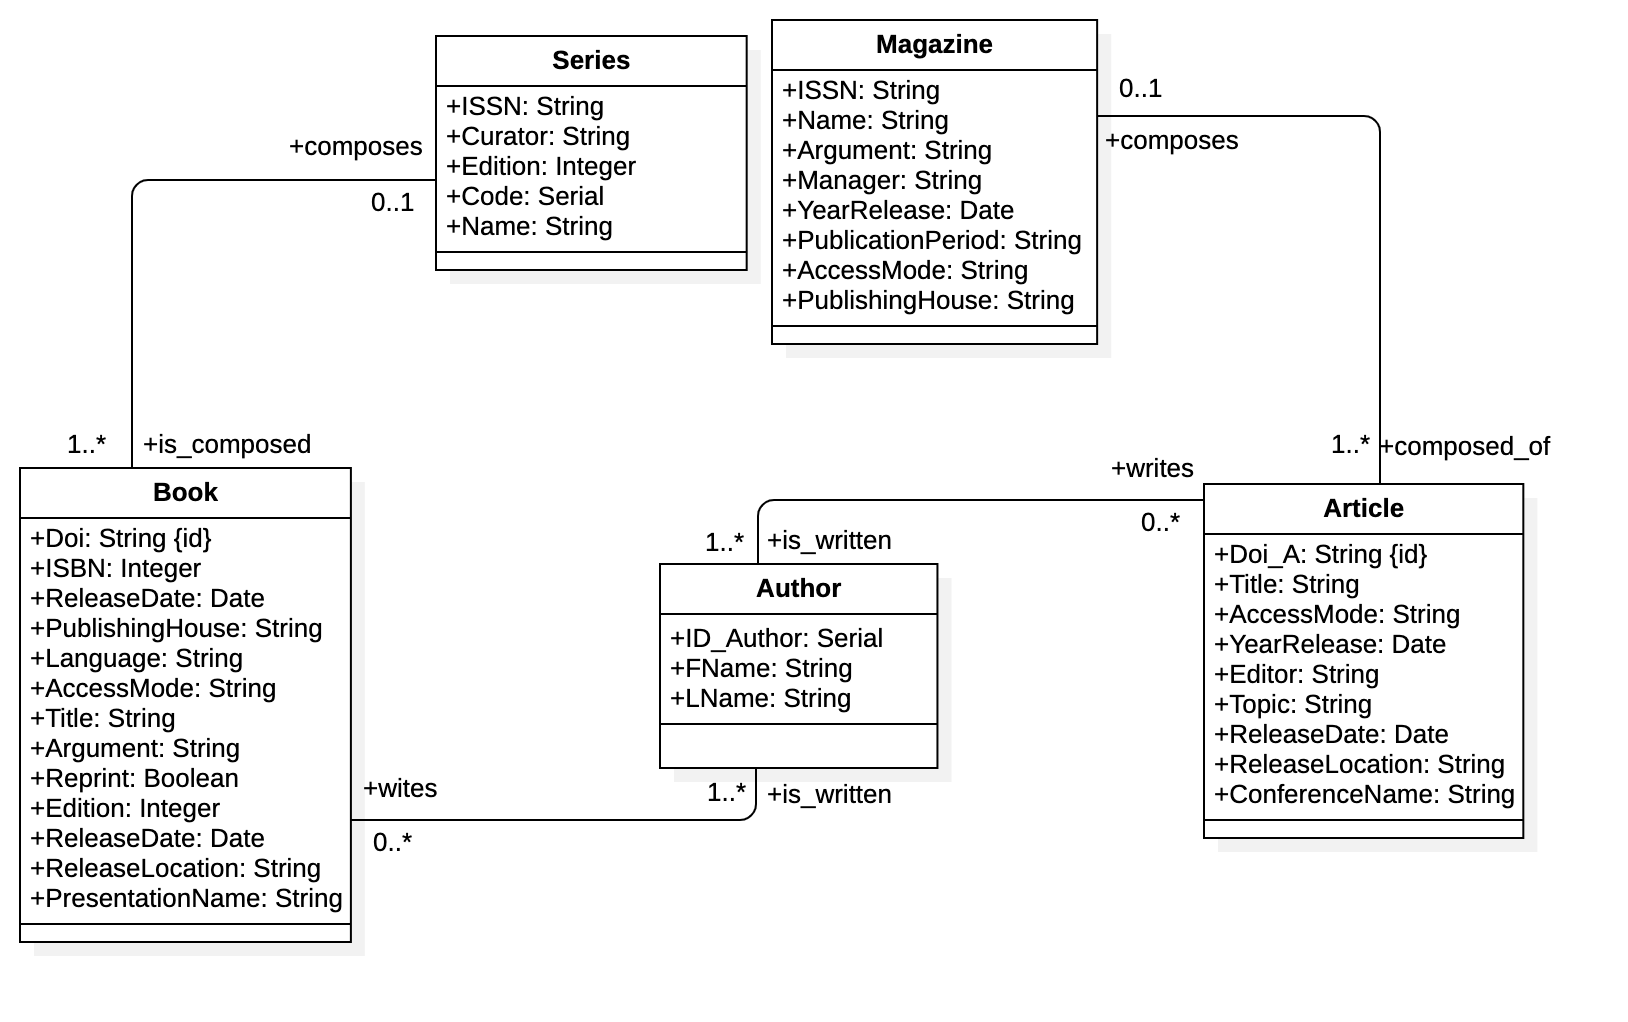
\includegraphics[width=1\textwidth]{Immagini/ClassDiagramRIS.png}
\caption{Class Diagram \\ Ristrutturato}
\label{fig:ClassDiagramRIS}
\end{figure}

\newpage
\begin{table}[]
\section{Dizionario delle Classi}
\caption{Dizionario delle Classi}

\label{tab:DizionarioClassi}

\resizebox{\textwidth}{!}{%
\begin{tabular}{|l|l|l|}
\hline
\rowcolor[HTML]{E5150C} 
Classe &
Spiegazione &
Attributi \\ \hline
\textbf{Author} &
Autore di libri o articoli &
\begin{tabular}[c]{@{}l@{}}ID\_Author (Serial): Identificazione dell'autore. \\ FirstName (String): Nome dell'autore. \\ LastName (String): Cognome dell'autore.\end{tabular} \\ \hline
\textbf{Books} &
\begin{tabular}[c]{@{}l@{}}Oggetti leggibili, romanzi o \\ d'educazione\end{tabular} &
\begin{tabular}[c]{@{}l@{}}
ISBN (Integer): Classificazione numerica di un libro. \\ Edition (Integer): Numero d'edizione. \\ AccessMode (AccessMode): Modo di fruizione. \\ ReleaseDate (Date): Data di pubblicazione. \\ PublishingHouse (String): Casa editrice che ha stampato il libo. \\ ReleaseLocation (String): Luogo di pubblicazione. \\ Language (String): Lingua in cui è scritto il libro.\\ Title (String): Titolo del libro. \\ Argument (String): Argomento del libro. \\ Reprint (Boolean): Parametro che identifica se il libro è una ristampa. \\ PresentationName (String): Nome della presentazione alla quale il libro è presentato.\end{tabular} \\ \hline
\textbf{Series} &
Insieme di libri &
\begin{tabular}[c]{@{}l@{}}ISSN (String):Numero internazionale che identifica le collane.\\ Edition (Integer):Numero dell'edizione. \\ Curator (String):Curatore della collana. \\ Code (Serial):Codice affidato alla collana. \\ Name (String): Nome della collana.\end{tabular} \\ \hline
\textbf{Magazine} &
Insieme di Articoli &
\begin{tabular}[c]{@{}l@{}}ISSN(Integer):numero internazionale che identifica le riviste. \\ Name (String): Nome della rivista. \\ Argument (String): Argomento della rivista. \\ Manager (String): Manager della rivista. \\ YearRelease (Timestamp): Anno di pubblicazione. \\ PublicationPeriod (String): Periodicità della rivista. \\ AccessMode (AccessMode): Modo di fruizione.\end{tabular} \\ \hline
\textbf{Article} &
Articoli di ricerca Scientifica &
\begin{tabular}[c]{@{}l@{}}DOI (String): Digital object Identifier dell'articolo.\\ Title (String): Titolo dell'articolo.\\ AccessMode (AccessMode): Metodo di fruizione.  \\ Editor (String):Editore dell'articolo. \\ ReleaseDate (Timestamp):Data di pubblicazione.\\ ReleaseLocation (String):Luogo di pubblicazione.\\ ConferenceName (String): Nome di conferenza in cui è presentato/discusso l'articolo.\end{tabular} \\ \hline
\end{tabular}%
}
\end{table}

\newpage

\begin{table}
\section{Dizionario delle associazioni}
\centering
\caption{Tabella delle Associazioni}
\resizebox{\linewidth}{!}{%
\begin{tabular}{|l|l|l|}	
\hline
\rowcolor[HTML]{E5150C} \multicolumn{1}{|r|}{Nome} & Descrizione                                                                                                                            & Classi Coinvolte  \\
composes/is\_composed                                        & \begin{tabular}[c]{@{}l@{}}Una collana è composta da uno o più libri/\\ Un libro può comporre oppure no una collana\end{tabular}       & Series/Book       \\ 
\hline
writes/is\_written                                           & \begin{tabular}[c]{@{}l@{}}Un libro è scritto da uno o più autori/\\ Un autore scrive molti oppure nessun libro\end{tabular} & Book/Author       \\ 
\hline
is\_written/writes                                           & \begin{tabular}[c]{@{}l@{}}Un autore scrive molti oppure nessun articolo/\\ Un articolo è scritto da uno o più autori\end{tabular}     & Author/Article    \\ 
\hline
composes/is\_composed                                        & \begin{tabular}[c]{@{}l@{}}Un articolo può comporre oppure no una rivista/\\ Una rivista è composta da uno o più articoli\end{tabular} & Article/Magazine  \\
\hline
\end{tabular}
}
\end{table}